\documentclass{article}
\usepackage[utf8]{inputenc}
\usepackage{amsmath}

\usepackage{hyperref}
\hypersetup{
    colorlinks=true,
    linkcolor=blue,
    filecolor=magenta,      
    urlcolor=cyan,
}

\usepackage{graphicx}

\setlength{\parindent}{0pt}

\title{Assignment-1 : Pattern Recognition}
\author{Arjun Manoharan (CS17S004) and Karthik Thiagarajan (CS16S027)}

\begin{document}

\maketitle

\tableofcontents

\newpage
\section{Singular Value Decomposition}
Singular Value Decomposition (SVD) \href{https://en.wikipedia.org/wiki/Singular_value_decomposition}{[1]} is one among several matrix factorization methods. We state the popular result for real matrices. Any $m \times n$ matrix $A$ can be expressed as the product of three matrices, $U$, $\Sigma$ and $V$:
$$
A = U \Sigma V^T
$$

where $U$ is an $m \times m$ orthogonal matrix consisting of the eigenvectors of $AA^T$, and $V$ is an $n \times n$ orthogonal matrix consisting of the eigenvectors of $A^TA$. $\Sigma$ is a rectangular $m \times n$  diagonal matrix consisting of the singular values of $A$. The singular values are nothing but the square roots of the eigenvalues of $A^TA$ and $AA^T$. The column vectors of $U$ are called the left singular vectors and the column vectors of $V$ the right singular vectors. The singular values are non-negative real numbers, usually written in the descending order. If the rank of a matrix is $r$, then the first $r$ singular values are non-zero \href{http://www.math.vt.edu/people/embree/cmda3606/chapter8.pdf}{[2]}.\\

The matrix can also be written in the following form:
$$
A = \sum \limits_{i = 0}^{r} \sigma_i u_i v_i^T
$$
where $u_i$ is the $i^{th}$ column of $U$, and $v_i^{T}$ is the $i^{th}$ row of $V$.\\

The above equation suggests a method to compute a compressed, approximate representation for a matrix. Using the first $k$ singular values, we can get an approximate matrix $\hat{A}$:
$$
\hat{A} = \sum \limits_{i = 0}^{k} \sigma_i u_i v_i^T
$$
The relative error in this approximation is computed using the Frobenius norm:
$$
e(\hat{A}, A) = \frac{\text{norm}(\hat{A} - A)}{\text{norm}(A)}
$$
where $\text{norm}(A) = \sum \limits_{i = 0}^{m} \sum \limits_{j=0}^{n} a_{ij}^{2}$

The first "$k$" singular values contain most of the information in the matrix, and can provide a good approximation. In our problem, the matrix we are concerned with is an image. 

\subsection{Grayscale}
This section will have the results for both square and rectangular matrices.

\subsubsection{Square Matrix}

We discuss experiment with two methods of picking the singular values. The first is to pick the top-N singular values. The other method is to pick them at random.\\

\textbf{Random = False}\\

The first plot describes the variation of the singular values. The log-scale is used on the y-axis.

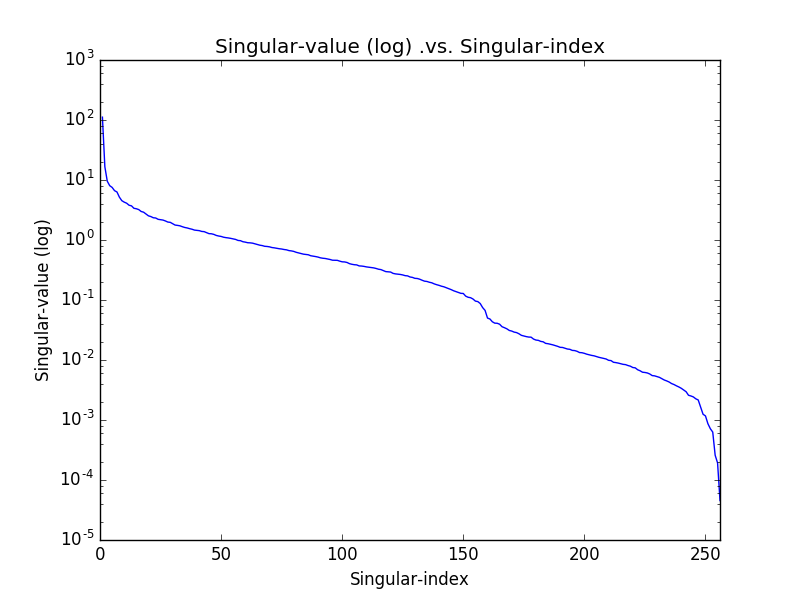
\includegraphics[width=\textwidth]{SVD/a/Square/False/singular.png}

We can see that the first $50$ singular values are greater than $1$. The last $100$ seem to be insignificant. The first $50$ singular values might help us get a decent reconstruction.

Next we reconstruct the images by picking the top-N singular values. The results for a few cases are shown:\\

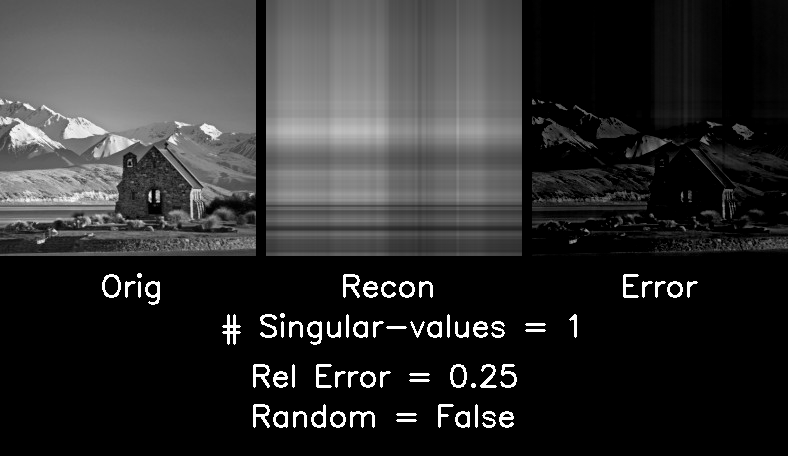
\includegraphics[width=\textwidth]{SVD/a/Square/False/recon0001.png}\\

The top-most singluar value is used here. Since $\hat{A}$ is a matrix of rank $1$, all the $256$ rows and columns can be expressed as the multiple of one row and one column respectively. This is observed as the horizontal and vertical patterns in the reconstrucrted image. Also note that the error image is almost the same as the original image.\\

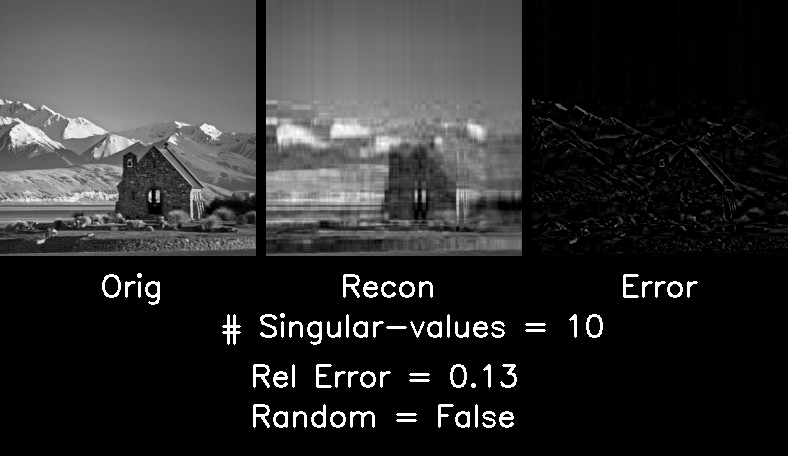
\includegraphics[width =\textwidth]{SVD/a/Square/False/recon0010.png}\\

With just $10$ singular values we are able to get most of the relevant features in the image. We are able to see a house and the mountaintops in the background. This level of detail may satisfy a machine learning researcher, but a professional photographer will want more.\\

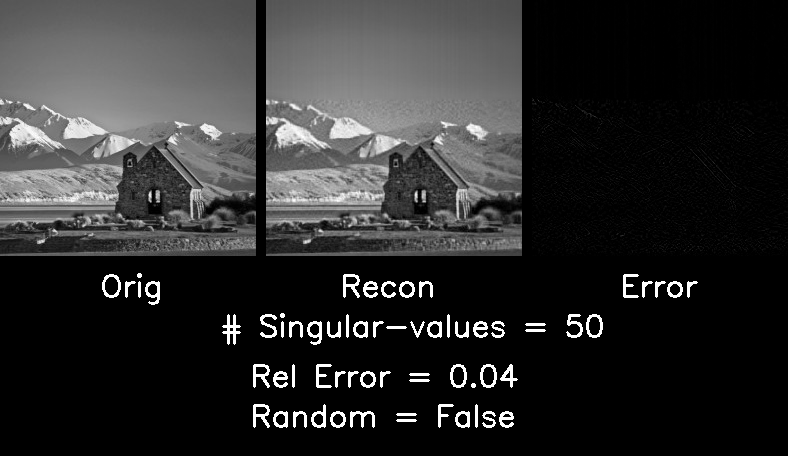
\includegraphics[width =\textwidth]{SVD/a/Square/False/recon0050.png}\\

With $50$ singular values we are almost there. A non-photographer will find nothing wrong with the reconstructed image. A very discerning observer may find some defect in the reconstruction. But a machine learning scientist will be more than satisfied. We have reduced $256 \times 256 = 65536$ float values into $2 * 50 * 256 + 50 = 25650$ float values, a compression ration of $2.5$!\\

What happens if we add the remaining singular values?\\

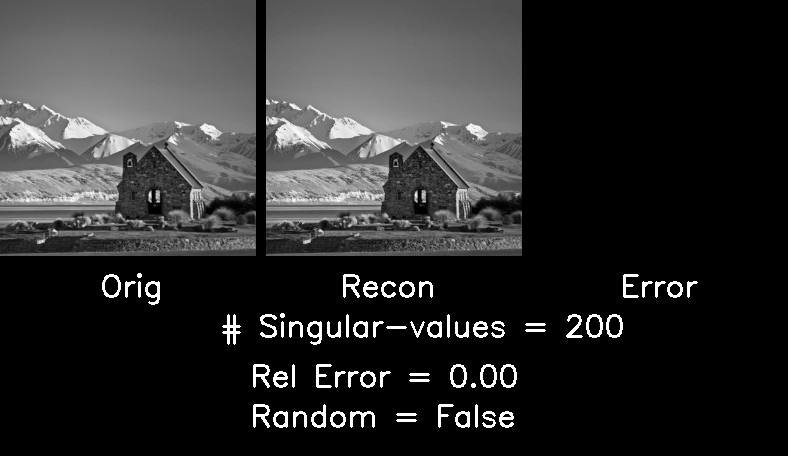
\includegraphics[width =\textwidth]{SVD/a/Square/False/recon0200.png}\\

Even our discerning observer will not be able to distinguish the original from the reconstructed image!

The next question concerns the variation of the reconstruction error agains the number of singular values used in the reconstruction.\\

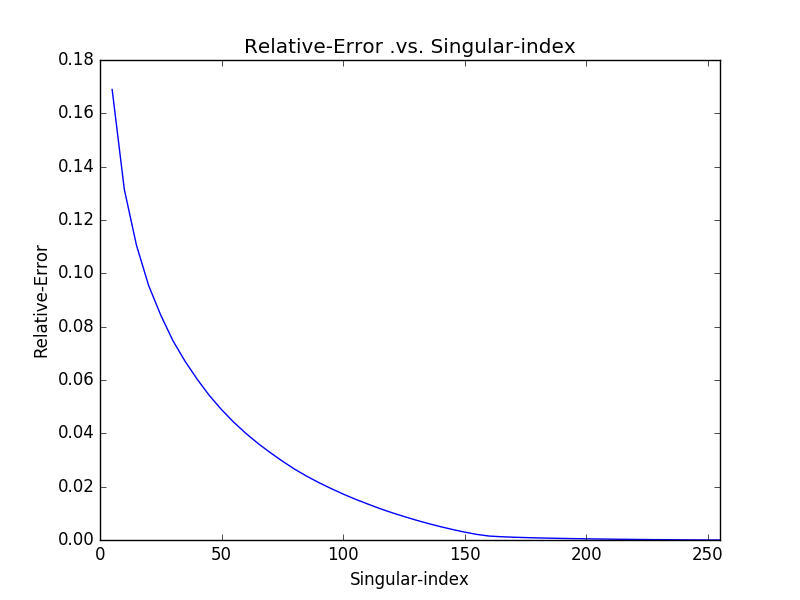
\includegraphics[width =\textwidth]{SVD/a/Square/False/error.png}\\

The trend is as expected. As we keep adding more singular values, different features of the image are captured, and the reconstruction progressively tends to the original.

\newpage
\textbf{Random = True}\\

We show a few reconstructions when singular values are picked at random:\\

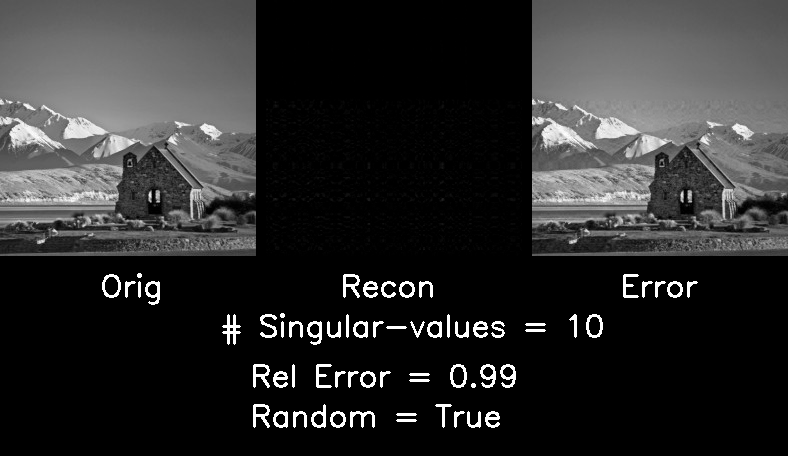
\includegraphics[width =\textwidth]{SVD/a/Square/True/recon0010.png}\\
With $10$ singular values, we were getting something more than just a black image in the previous case. Thus the magnitude of the singular values matter. The first few singular values hold most of the information in the image.\\

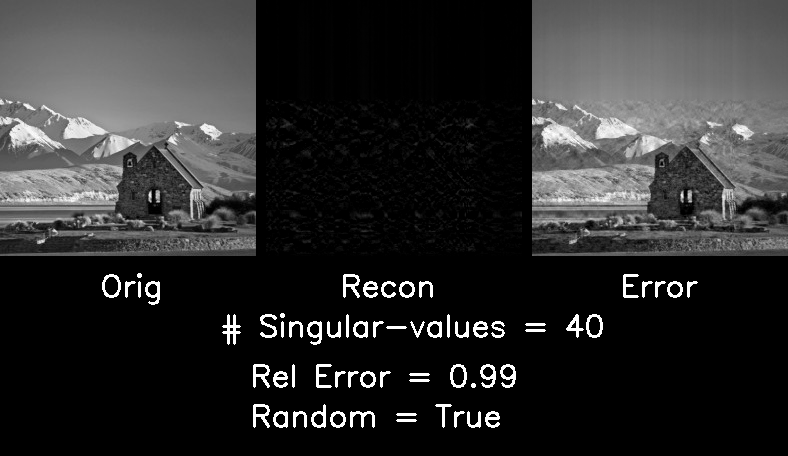
\includegraphics[width =\textwidth]{SVD/a/Square/True/recon0040.png}\\

This reiterates the above statement.\\

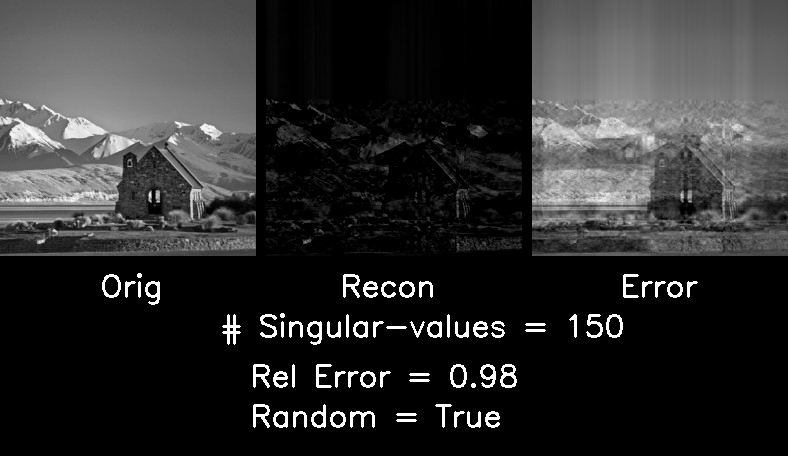
\includegraphics[width =\textwidth]{SVD/a/Square/True/recon0150.png}\\

Even as many as $150$ singular values are not sufficient. This is quite obvious. From the first experiment we know that the first 50 singular values hold most of the information, these $150$ may not contain the most important ones.\\

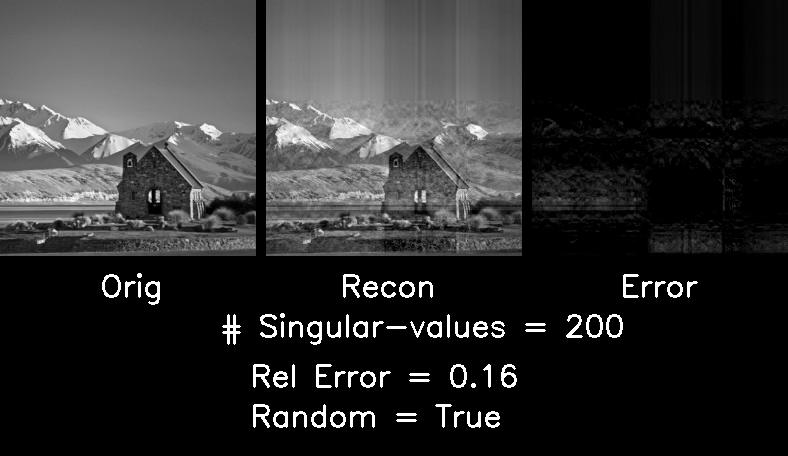
\includegraphics[width =\textwidth]{SVD/a/Square/True/recon0200.png}\\

Next is the plot of the error versus the number of singular values chosen:\\

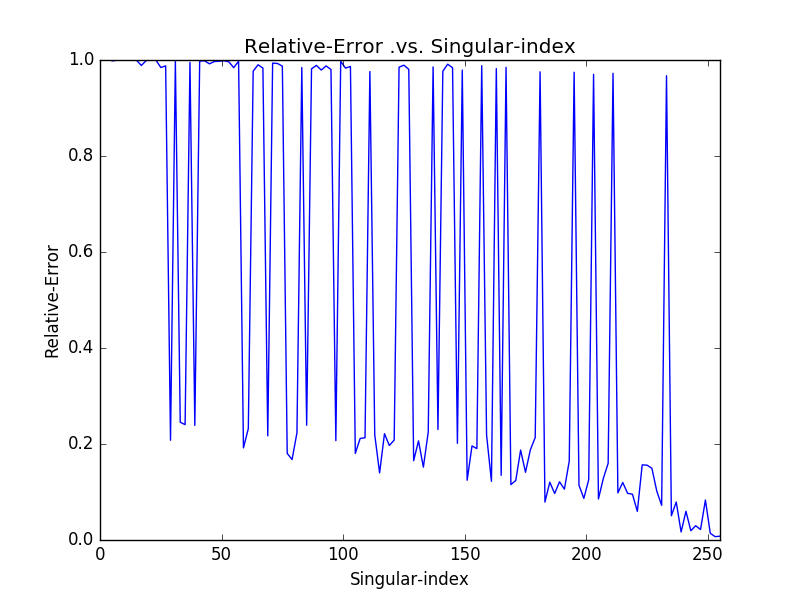
\includegraphics[width =\textwidth]{SVD/a/Square/True/error.png}\\

What could be the reason for the wild oscillations that are observed here? Every time the graph attains a crest, or a low reconstruction error, then the random collection of singular values contains the first few of the most important ones. Whenever there is a peak, the random collection has missed most of the top few singular values. The oscillations remain well until the number $225$. This makes sense since the number of important singular values is less than $50$, to be absolutely sure of getting at least few of the important singular values, one needs to pick at least $200 + k$ of them.

Another interesting observation is the height of the peak. Initially it is close to 1, and then progressively decreases. 

\newpage
\subsubsection{Rectangular Matrix}

The first set of experiments will be for the top-N singular values.\\

\textbf{Random = False}\\

The first plot shows the variation of the singular values.\\

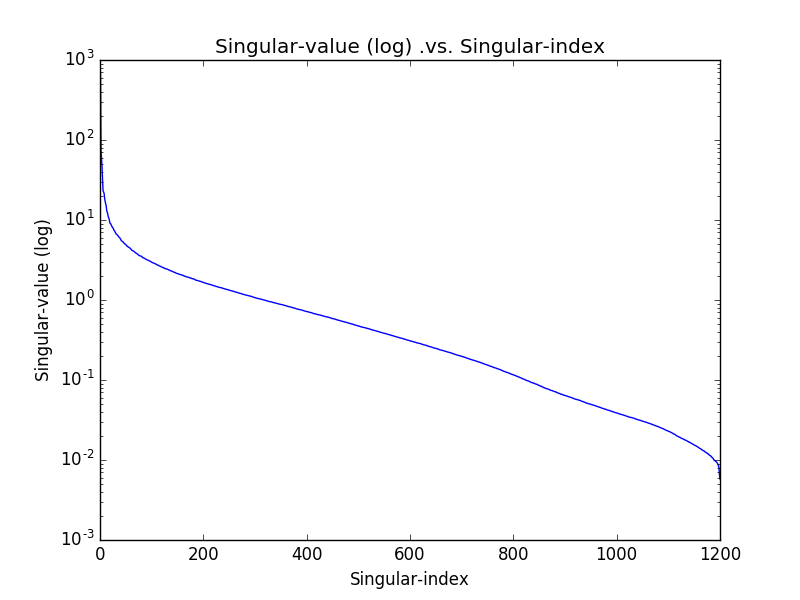
\includegraphics[width =\textwidth]{SVD/a/Rect/False/singular.png}\\

There are $1200$ singular values, all non-zero. The first $200$ are above $1$. As in the previous case, we can hope to get a good reconstruction with just these $200$ values.\\

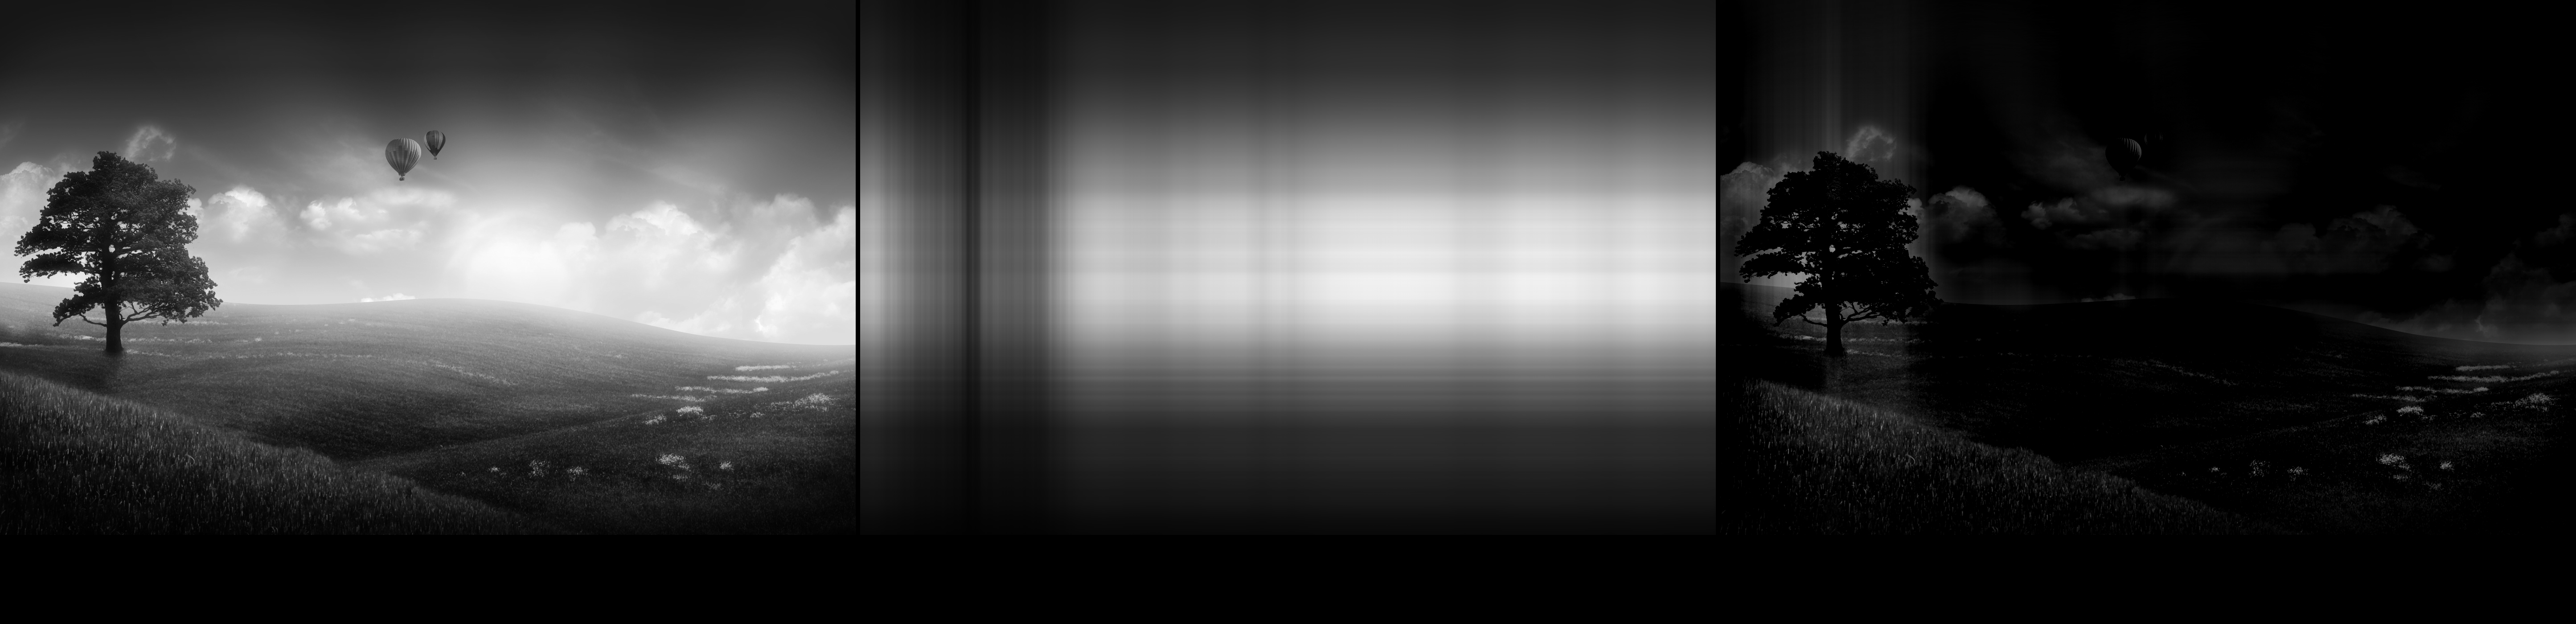
\includegraphics[width =\textwidth]{SVD/a/Rect/False/recon0001.png}\\

The above plot is with the first singular value, this is the rank-1 matrix as before.\\

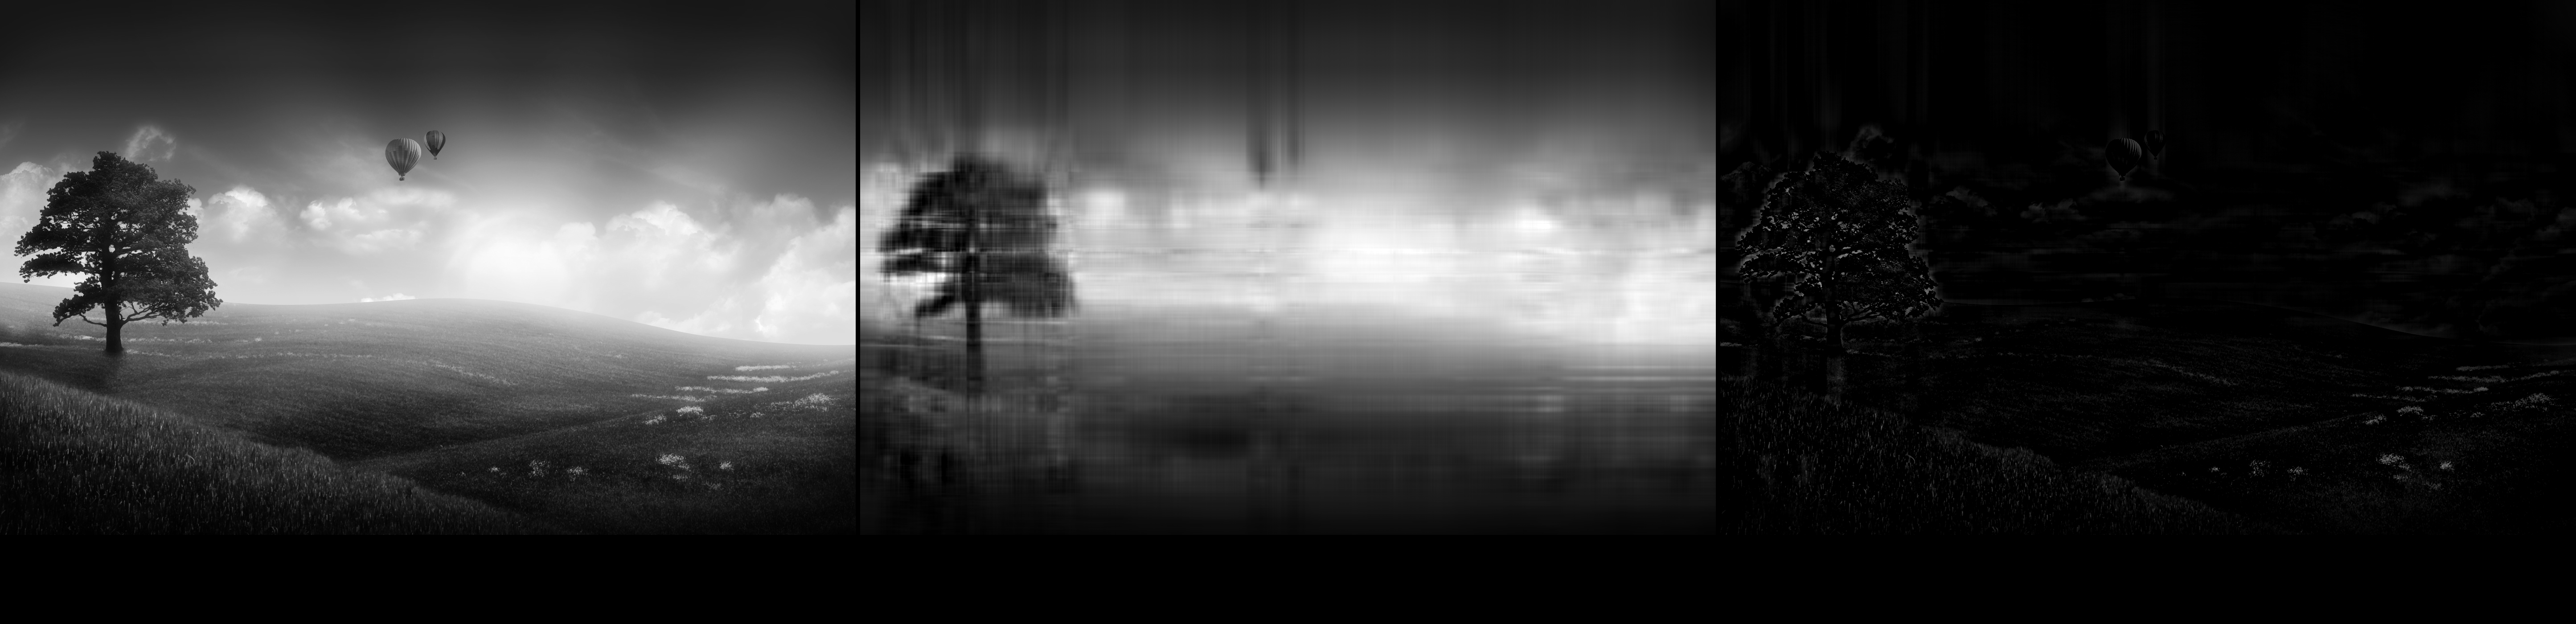
\includegraphics[width =\textwidth]{SVD/a/Rect/False/recon0010.png}\\

The above plot is with $10$ singular values. There is a surprising level of clarity. The balloons in the background are not visible, though.\\

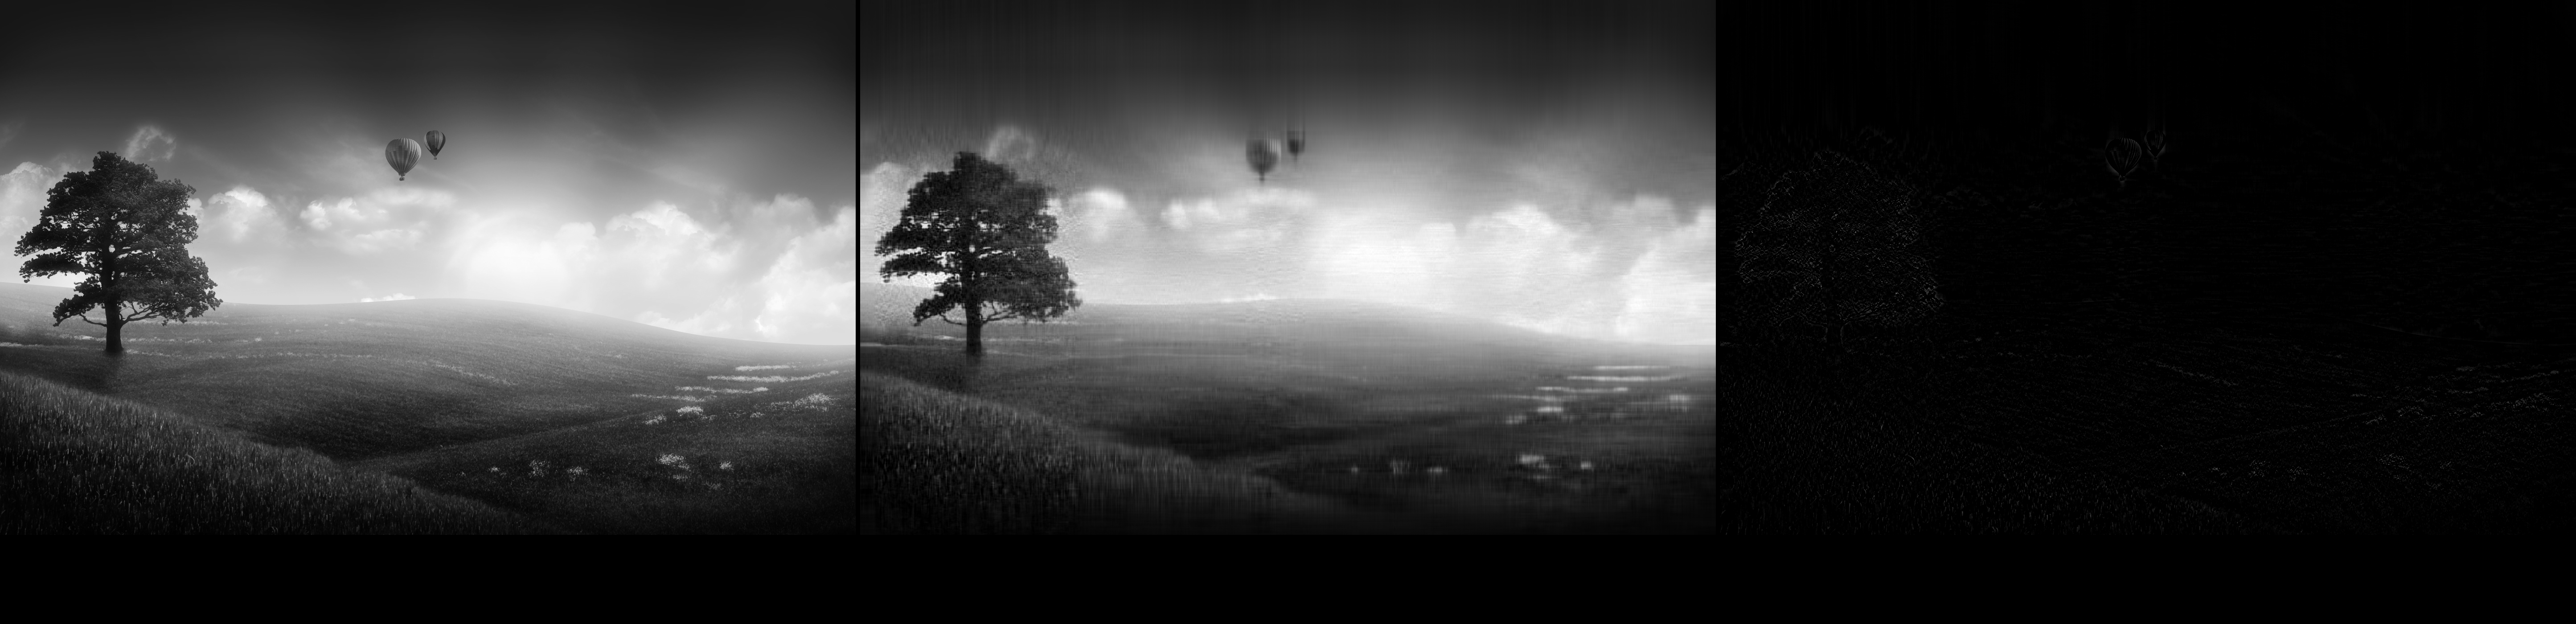
\includegraphics[width =\textwidth]{SVD/a/Rect/False/recon0050.png}\\
The above plot is with $50$ values. We are almost there. The error image is almost black.\\

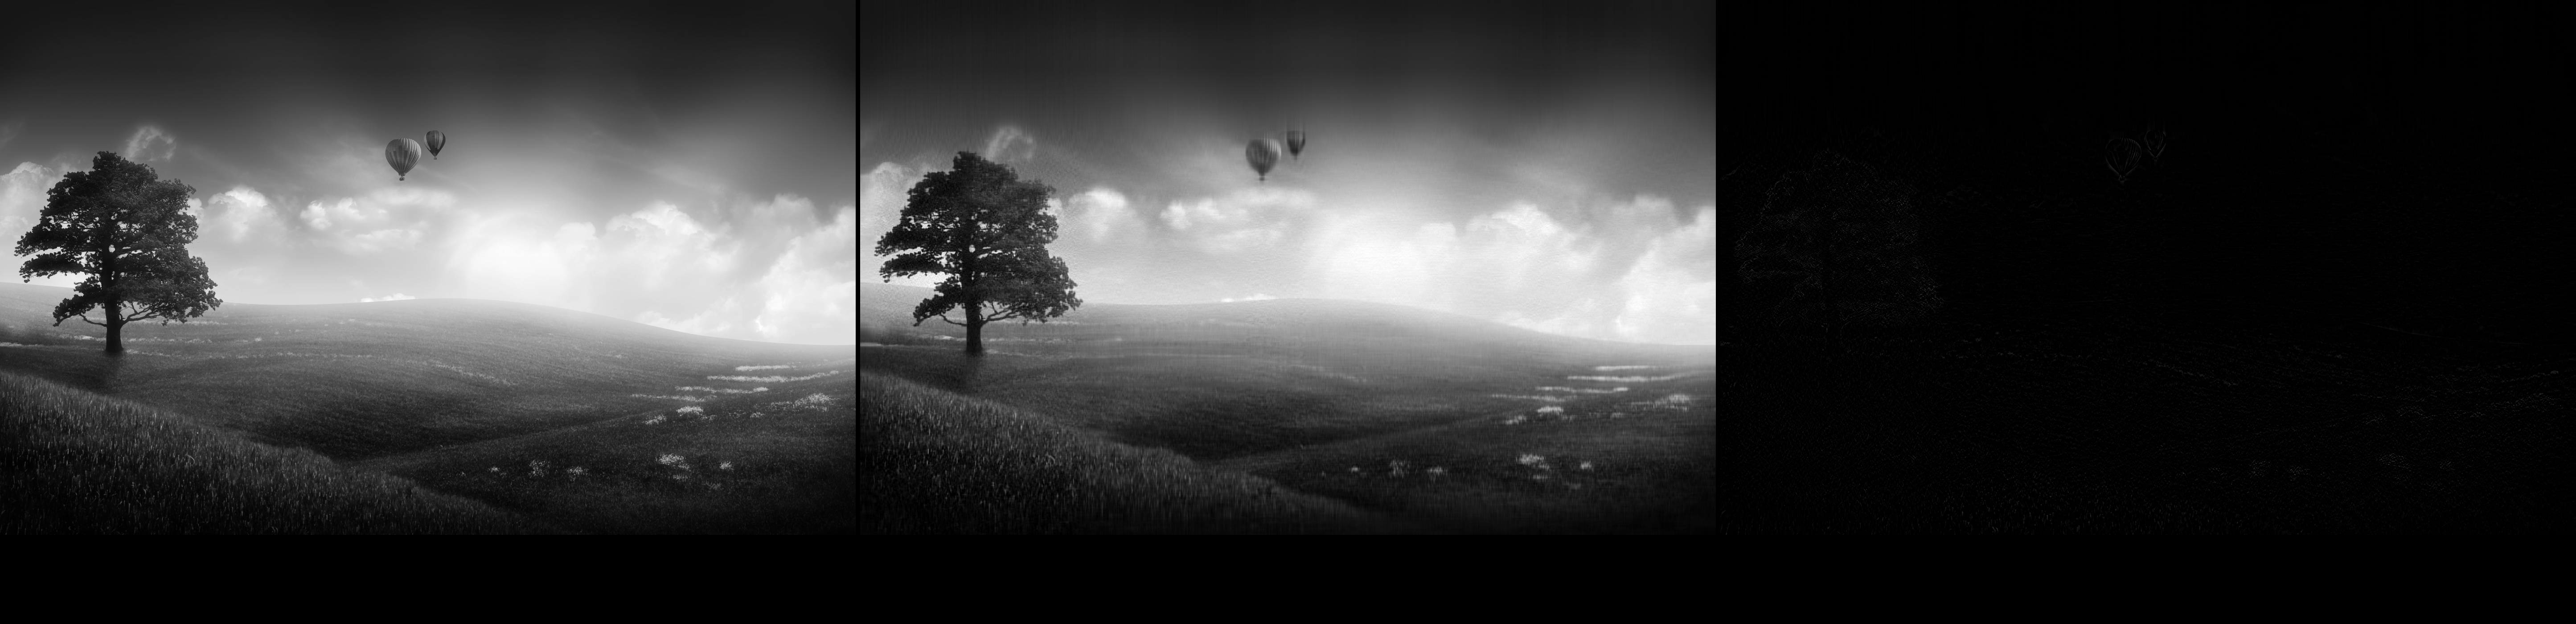
\includegraphics[width =\textwidth]{SVD/a/Rect/False/recon0100.png}\\
The above plot is with $100$ values.\\


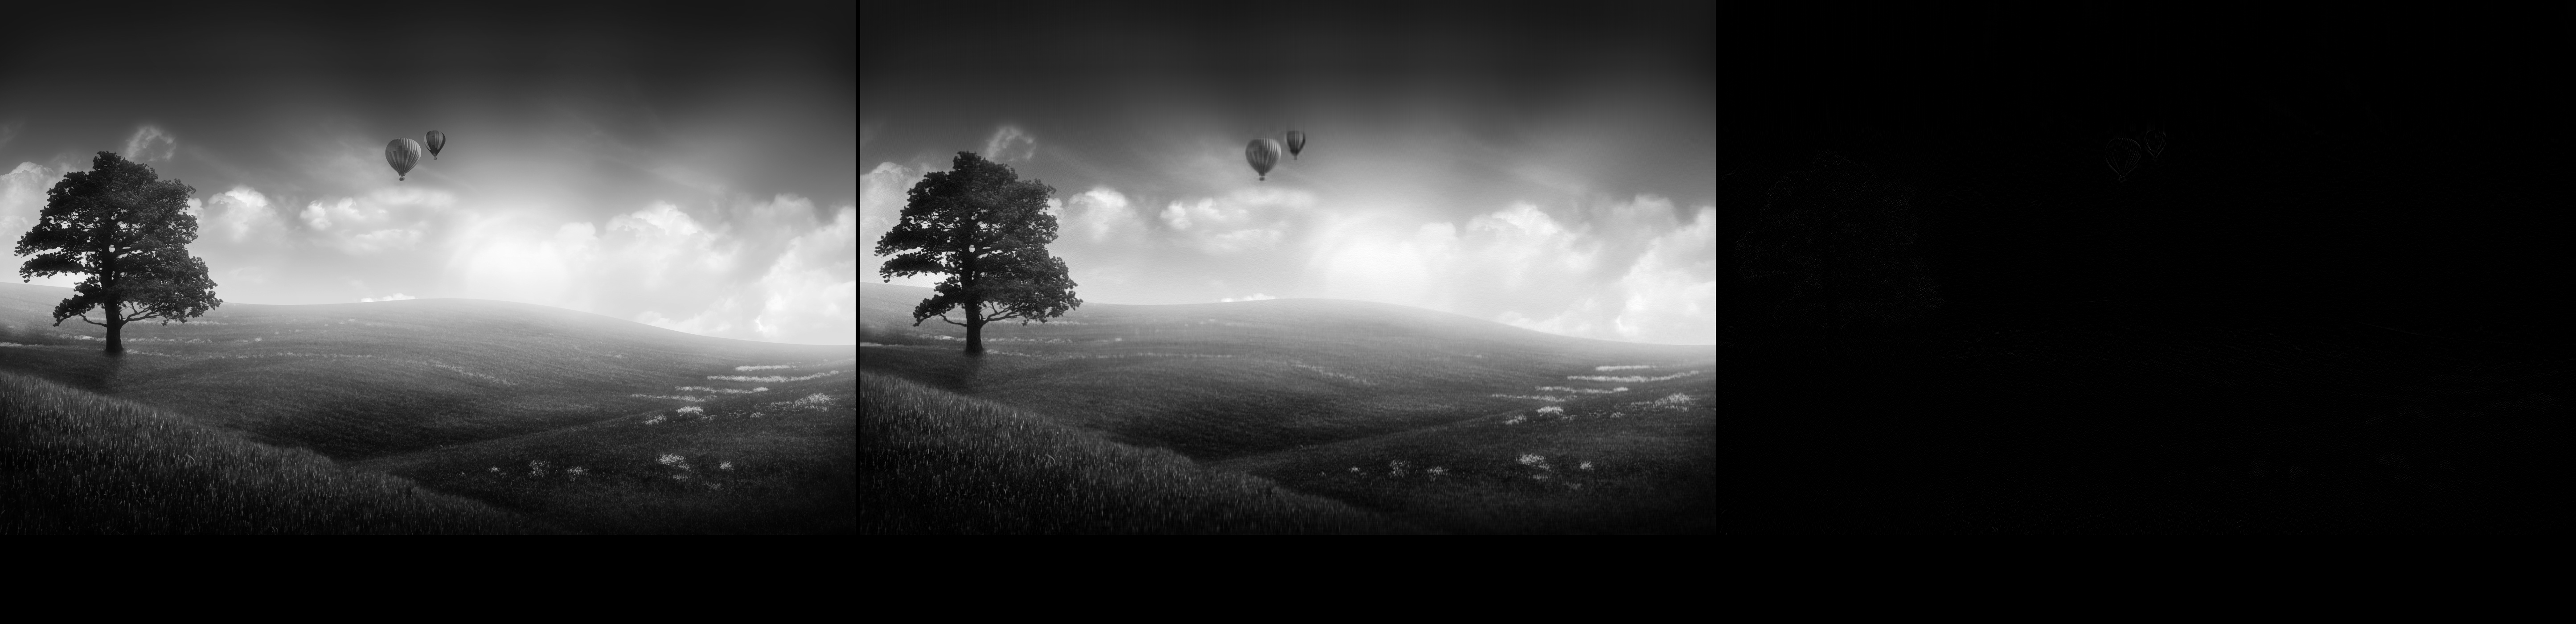
\includegraphics[width =\textwidth]{SVD/a/Rect/False/recon0200.png}\\
The above plot is with $200$ values.\\

There is a very nice thing about these plots. The amount of detail that was added in the reconstructed image from singular values $1$ through $50$ is far greater than the amount of detail that was added from $50$ to $200$. This perfectly aligns with the plot. The slope is very steep until the $50^{th}$ singular value. From there it starts becoming more and more horizontal.\\

A plot of the error is shown below:\\

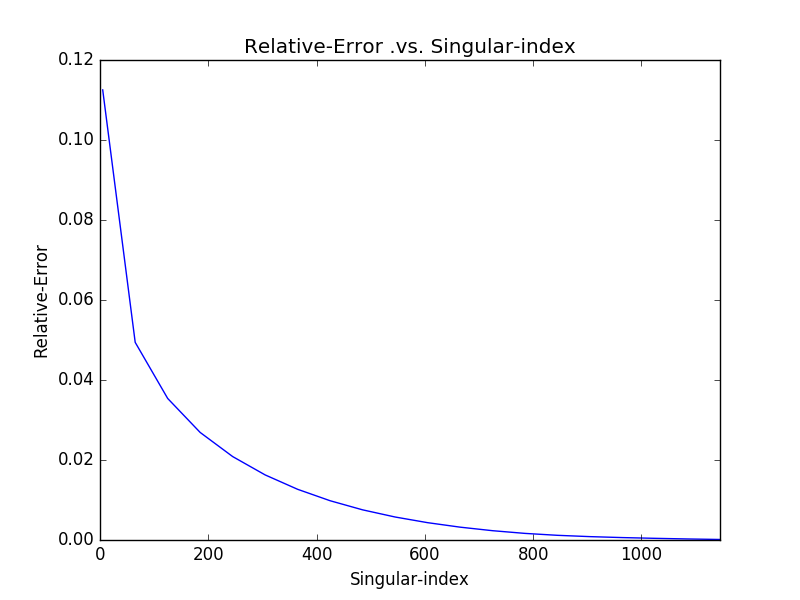
\includegraphics[width =\textwidth]{SVD/a/Rect/False/error.png}\\

The cuve looks linear during the first $50$ values with a steep slope. From there it starts to decrease slowly to zero.\\

How much do we save in terms of memory?\\
The original image has $1920 * 1200 = 2304000$ float values. With $50$ singular values, we need to store $50 * (1920 + 1200) + 50 = 156050$. This gives us a factor of reduction equal to $14$. Quite good! 


\newpage
\textbf{Random = True}

A few reconstructions are shown here:\\

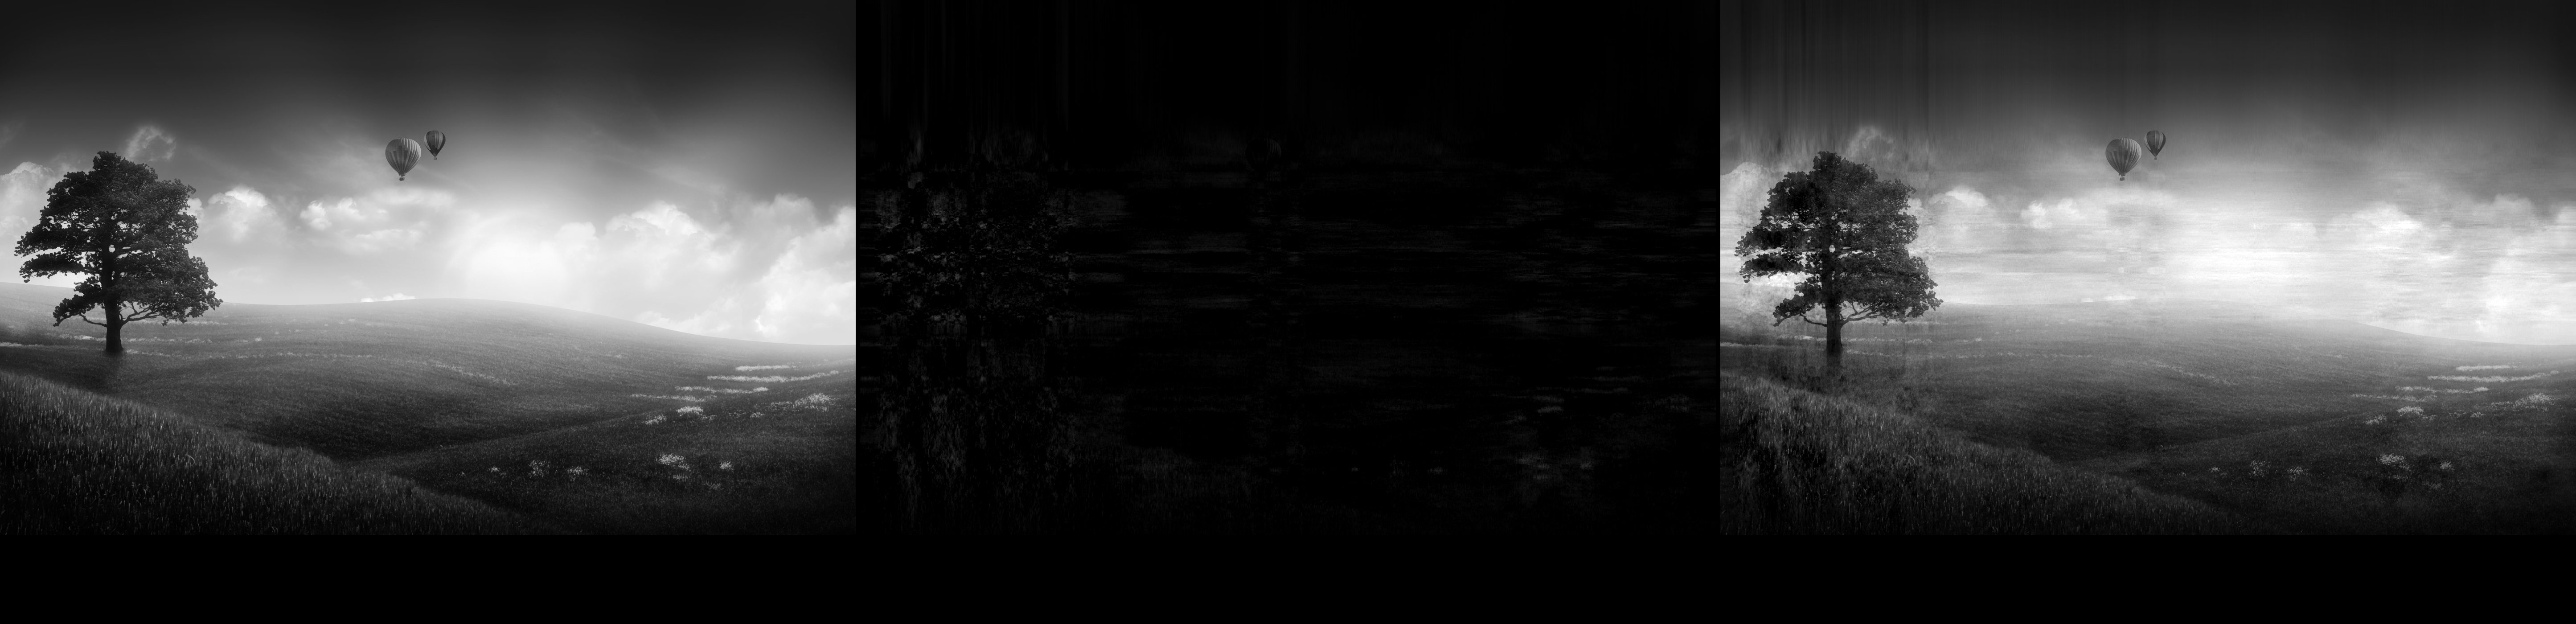
\includegraphics[width =\textwidth]{SVD/a/Rect/True/recon0200.png}\\
The above one is for $200$ singular values.\\

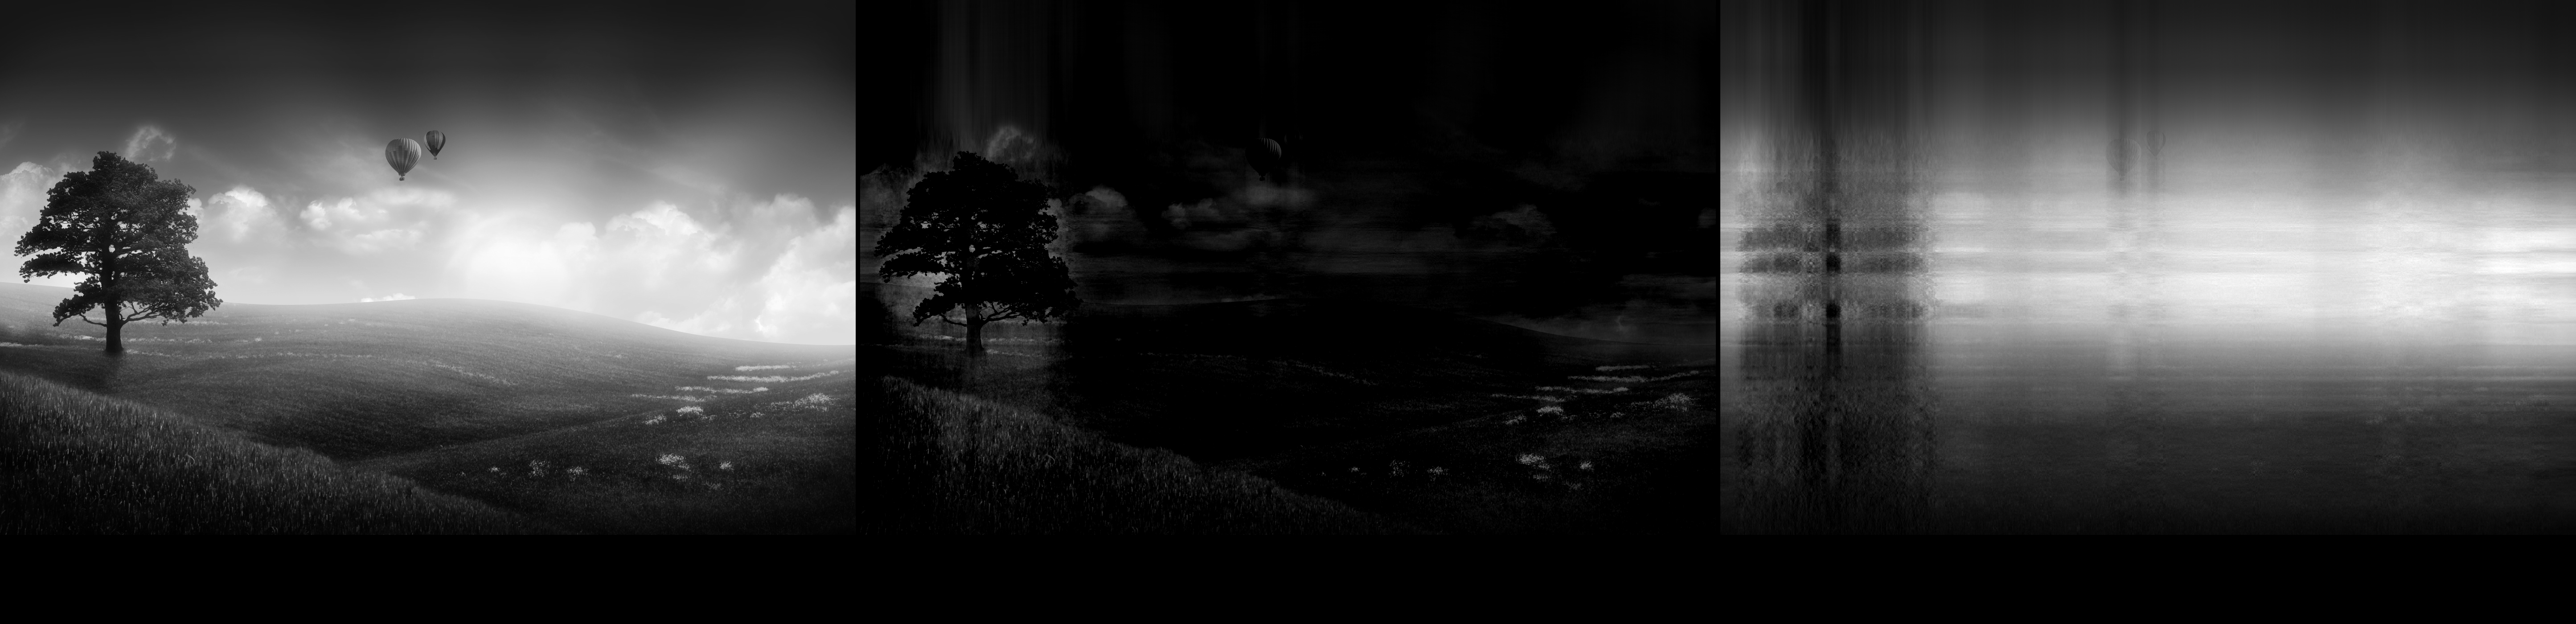
\includegraphics[width =\textwidth]{SVD/a/Rect/True/recon1000.png}\\
The above one is for $1000$ singular values.\\

The same conclusion holds as for the square case. We need at least $1200 - 50 + k$ singular values picked at random to get a good reconstruction. The error plot is as given below:\\
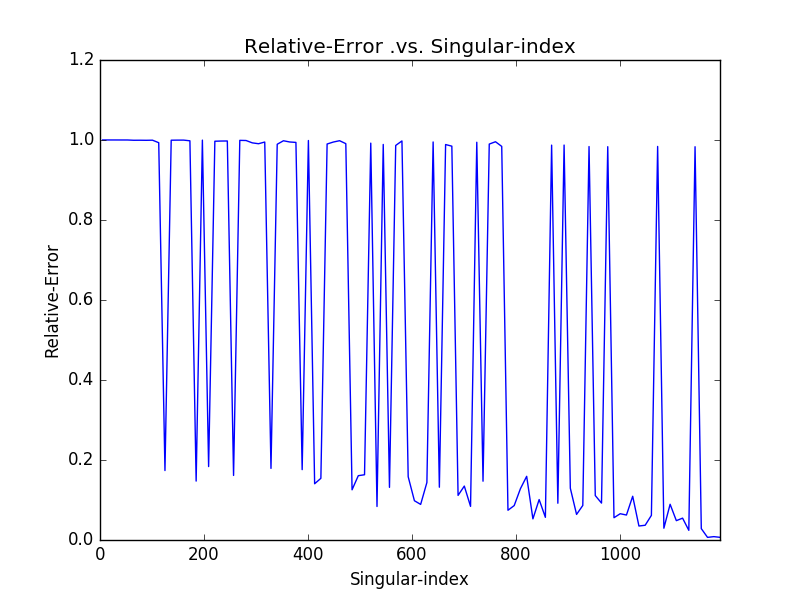
\includegraphics[width =\textwidth]{SVD/a/Rect/True/error.png}\\

Note that the peak is very close to $1$ right till the end. This is understandable since we are dealing with a large number of singular values ($1200$), yet the number of significant singular values remains the same, approximately $50$. Thus the probability of picking the top-50 singular values comes down.


\newpage
\subsection{Independent Channels}

\newpage
\subsection{Concatenating Channels}


\newpage
\section{Eigenvalue Decomposition}

The eigenvalue decomposition is the factorization of the matrix using its eigenvalues and eigenvectors. For a square, $n \times n$ matrix $A$,
$$
A = Q \Lambda Q^{-1}
$$
where $\Lambda$ is a diagonal matrix with the eigenvalues of $A$ as its entries, and $Q$ contains the corresponding eigenvectors as its columns. If the underlying field is the complex space, then every real or complex matrix has this decomposition. If the underlying field is real, then only those matrices that have characteristic equations that split can be written in this form.


\subsection{Grayscale}

\subsubsection{Square Image}


\section{Polynomial Regression}


\subsection{One-dimesnional data}

\subsection{Two-dimensional data}

\subsection{Multi-dimensional data}


\end{document}

